%%
% Einbinden der Dokumentklasse
\documentclass[12pt]{article}
%%
% Einbinden der Packages
\usepackage{german}
\usepackage{a4wide}
\usepackage{ngerman}
\usepackage[latin1]{inputenc}
\usepackage{graphicx}
\usepackage{setspace}
\usepackage{chngpage}
\usepackage{listings}
%\usepackage{float}
%\usepackage{floatflt}
\usepackage{pst-3dplot}
\usepackage{epsfig} 			%  f�r eps graphiken
\usepackage[ngerman]{babel}
\usepackage{bbm}
%\usepackege{amssymb}
%%
% Einstellen 1,5fachen Zeilenabstand
\onehalfspacing

\title{Facharbeit -  Coumputer Simulation von geladenen Teilchen im elektrischen und magnetischen Feld} 
\author{Matthias Lochbrunner}
\date{\today}

%%
% Start des Dokumentes
\begin{document}

%	\pdfinfo { 
%  	/Title (Coumputer Simulation von geladenen Teilchen im elektrischen und magnetischen Feld) 
%  	/Creator (PDFLaTeX) 
%  	/Producer (SKG-Krumbach) 
%  	/Author (Matthias Lochbrunner) 
%  	/CreationDate (\today) 
%  	/ModDate (\today) 
%  	/Subject (Facharbeit 2007-2008) 
%  	/Keywords (Facharbeit) 
%	}

	%%
	% Einbinden Titelseite
	%%%%%%%%%%%%%%%%%%%%%%%%%%%%%%%%%%%%%%%%%%%%%%%%%%
%% titelseite.tex																%%
%%%%%%%%%%%%%%%%%%%%%%%%%%%%%%%%%%%%%%%%%%%%%%%%%%
%% In dieser Datei werden die Einstellungen zur %%
%% Titelseite gemacht														%%
%%%%%%%%%%%%%%%%%%%%%%%%%%%%%%%%%%%%%%%%%%%%%%%%%%

% Einstellung ohne Seitennummerierung
\thispagestyle{empty}

% Einstellen des Erstzeileneinzugs
\setlength{\parindent}{0pt}

% fetter Text, Kopf der Seite
\textbf{Simpert-Kraemer-Gymnasium \hfill 2006/2008 \\
Krumbach}

% vertikal f�llen
\vfill


\begin{center}
  \textsc{\Huge{Bedienungsanleitung}}\\  
  \large{f�r eine Computersimualtion aus dem Bereich der }\\ 
  \vspace*{.3cm}
  
  %%
  % Hier Fach eintragen
  \textsc{\Huge{Physik}}
  
\end{center}

% vertikal f�llen
\vfill

\begin{large}
  \textbf{Name:}  
  %%
  % Hier Thema eintragen
  Computersimulation von geladenen Teilchen im elektrischen und magnetischen Feld
  
\end{large}
\vfill

%%
% Name, Fach, Lehrer und Datum eintragen
\begin{tabular}{ll}
  Verfasser:    & Lochbrunner Matthias\\
  Leistungskurs:& Physik \\
  Erstellt am: &  \today
\end{tabular}

% vertikal f�llen
\vfill



	%%
	% Inhaltsverzeichnis
	\tableofcontents
	
	\thispagestyle{empty}


	% Keine Nummerierung im Inhaltsverzeichnis
	\thispagestyle{empty}

	\newpage
	% Einstellen des Textlayouts auf Vorgaben f�r Facharbeiten
		\setlength{\hoffset}{-1in}
		\setlength{\voffset}{-1in}
		\setlength{\textwidth}{0cm}
		\changetext{3cm}{15cm}{2cm}{4cm}{}
		\setlength{\topmargin}{1.4cm}
	
	%%
	% Einbinden des Haupttextes
	\section {Einf�hrung zum Thema}
 
Zu Zeiten Isaac Newtons war die Physik noch ein sehr �berschaubares Gebiet der Wissenschaft. Als Rechenhandwerk gen�gten primitivste Differenzial- und Integralrechnung vollkommen. Gleichungen dritten Grades waren eine Seltenheit. Und war mal ein neuartiges Ph�nomen gefunden, dass mit den bekannten Gesetzen nicht beschrieben werden konnte, bot sich immer noch die M�glichkeit die fehlende Erkenntisse durch ein Experiment zu erlangen. Der Einfallsreichtum unter den Versuchsaufbauten war oftmals erstaunlich.
Doch sp�testens seit dem ersten Versuch, einen Menschen auf den Mond zu schie�en, w�re es ein recht teueres Unterfangen gewesen eine Vielzahl von Raketen gen Himmel zu schicken nur um herauszufinden, wie stark die Triebwerksk�pfe sein m�ssten um das Vehikel zur gew�nschten Umlaufbahn zu bef�rdern. Hier wurde dann auch erstmals das Berechnen von Koordinaten und Kreisbahnen mit Papier und Bleistift ein Ding der Unm�glichkeit. Nicht nur weil die Rechnungen eines einzelnen Teilabschnittes unerm��lich lang und  aufw�ndig wurde, sondern auch weil niemand die Verantwortung �bernehmen wollte, wegen einem Rechenfehler ein Menschenleben zu riskieren.
Ein neuer Weg musste gefunden werden, solch komplexe Berechungen schnell und exakt durchf�hren zu k�nnen. Man mag die Wissenschaftler wohl noch ausgelacht haben, als sie mit Lochstreifen bewaffnet den ersten R�hrenrie�en das multiplizieren beibrachten um ihnen nach monatelangem gut Zureden dazu zu bringen, die Kurven m�glicher Flugbahnen auszuspucken.
Diese Hilfe verwendet man heute auch "`in der Elementarteilchenphysik, in der Materialforschung, Str�mungsdynamik, Strukturmechanik, Chemie, Geo- und Astrophysik sowie Klima- und Umweltforschung"'\footnote{Quelle : http://www.stmwfk.bayern.de/pressearchiv/meldung.asp?NewsID=649}.
Dazu reichen heutzutage allerdings keine Triodenrechner mehr, die in einer Sekunde eine Handvoll Rechenschritte durchf�hren, sondern es werden meist Gro�rechner wie der Leibnizrechner in Garching ben�tigt, um die rie�ige Datenflut und die �beraus komplizierten Berechnungen, die dennoch nur Ann�herungen sind, zu bew�ltigen.\\
Aber auch im Kleinen lassen sich durch Computersimulationen viele physikalische Ph�nomen anschaulich erkl�ren. Eine gro�e Hilfe f�r Physiklehrer, die im Unterricht bei Sch�lern oft auf Unverst�ndis und mangelnder Vorstellungskraft treffen.
Die Vorteile des Computereinsatzes im Unterricht liegen klar auf der Hand: So lassen sich durch eine geeignete Simulation das komplexe Zusammenspiel vieler Umwelteinfl�sse auf einzellne wichtige Faktoren begrenzen und diese komplizierten Sachverhalte durch transpatente Modelle durchleuchten, da unn�tige Einfl�sse ausgeblendet werden. Idealbedingungen k�nnen geschaffen werden. Auch erm�glichen diese das beobachten physiklaischer Experimente die real im Unterrricht niemals durchf�hrbar w�ren, wie zum Beispiel sehr langsame bzw. sehr schnell ablaufende Effekte wie ein elektischer Blitz, ebenso Versuche mit strahlenden oder hoch giftigen Materialien w�ren im Klassenzimmer unverantwortlich mit einem Computersimualtion jedoch anschaulich durchf�hrbar\footnote{Quelle : http://www.medien.ifi.lmu.de/fileadmin/mimuc/mll\_ws0506/Vortrag\_Kim.pdf}.
Zwar bietet das Internet ein reichhaltiges Angebot physikalischer Simualtionsprogramme, oft sogar als Java-Applet oder Flash-Skript direkt im Internetbrowser ausf�hrbar, doch nur die Wenigsten von ihnen arbeiten mit der dritten Dimension, und alle haben nur einen beschr�nkten Anwendungsbereich. Da sie meist nur geskriptet sind, bekommt der Betrachter quasi nur einen Film vorgesetzt, bei dem er manche Werte mit Reglern verstellen kann. Diese Nische zu f�llen entschied ich mich, selber im Rahmen dieser Facharbeit, ein Programm zu entwickeln, das auf der Basis von Microsoft DirectX\texttrademark geschrieben in \textsl{C++}, phyikalische Ph�nomene in den Bereichen Elektrostatik und Magnetismus im dreidimensionalem Raum simulieren kann.
Hierf�r setze ich auf das bewerte Editor-Prinzip, welches dem Anwender erlaubt sich aus einer Reihe von Bausteinen seine gew�nschte Szene zusammen zu stellen, genauso wie es in komerziellen 3D-Simulationen wie Maya oder Cinema3D �blich ist.
Somit lassen sich dann die Verhaltensmuster Elementarteichen in bestimmten Umgebungen beobachten; genauere Ph�nomene werden am Schluss dieser Arbeit behandelt. Zun�chst werde ich kurz die Handhabung und den Umfang des Programms vorstellen, danach noch auf die physikalischen Gesetze eingehen, die in dieser Simulation Anwendung finden und wie sie im Code umgesetzt wurden.
Die Angabe genauer Ergebisse und realit�tsgetreuer Werte, die genau berechnete Konstanten im Quellcode vorraussetzt, ist nicht Aufgabe dieser Facharbeit. Und somit handelt es sich um eine reine Simulation ohne Messm�glichkeit.\\

	\section{Kurze Bedienungsanleitung}

\subsection{Installation}

Vor der Installation sollte sichergestellt sein, dass auf dem PC ein lauff�higes "`Windows XP"' mit Service Pack 2 installiert ist und eine aktuelle Version der Hardwareschnittstelle "`DirectX 9.0c"' oder neuer bereits Verwendung findet. Da die Simulation bereits mit dem "`DirectX SDK"' von 2007 geschrieben wurde, empfiehlt es sich gegeben falls, die "`Runtime"' Version auf dem PC zu aktualisieren \footnote{Download : http://www.microsoft.com/downloads/details.aspx?displaylang=de\&FamilyID=2da43d38-db71-4c1b-bc6a-9b6652cd92a3}. \\
Nach Einlegen der CD in das Laufwerk erscheint automatisch ein mit "`Install Creater"' erzeugtes Installationsfenster. Sollte das Fenster nicht automatisch erscheinen, kann das Setup auf der CD auch manuell unter \textsl{/Software/Setup.exe} gestartet werden. Die Anweisungen des Installationsassistenten erkl�ren sich selbst. Nach erfolgreicher Installation erh�lt das Programm nun im \textsl{Startmen�}, unter \textsl{alle Progamme} einen Eintrag. 
Ebenfalls sind auf der CD noch weitere Dateien bez�glich dieser Facharbeit zu finden. So z.B. dieses Skript als pdf-Datei, sowie der Quellcode des Programms und noch zus�tzliche Materialien. Gegebenenfalls muss dazu die CD im \textsl{Arbeitsplatz} mit Rechtsklick, \textsl{�ffnen}, da bei einem Doppelkick der \textsl{autorun} der CD das Installationsprogramm starten w�rde.


\subsection{Freie Kamerabewegung}

Das Gedr�ckthalten der \textsl{Alt}-Taste signalisiert dem Programm, dass die Maus nun zur Steuerung der Kamera verwendet wird.
Jetzt l�sst sich mit der mittleren Maustaste die Szene parallel zur Sichtebene verschieben, wobei der Cursor ein anderes Symbol erh�lt, eines mit einem Pfeil in jede Himmelsrichtung. Um sich im Raum zu drehen wird die linke Maustaste verwendet. Jede Drehung erfolgt immer um einen bestimmten Mittelpunkt. Dieser ist entweder die Position des zuletzt markierten Elements in der Szene, oder falls nichts markiert wurde, der Ursprung im Koordinatensystem. Als Cursor erscheinen nun zwei im Kreis laufende Pfeile.
Der Zoom bzw. der Abstand der Kamera zur Szene wird mit der rechten Maustaste ver�ndert. Hier gilt: Wird die Maus nach links oben verschoben, wird aus der Szene herausgezoomt, beim Verschieben nach rechts unten hineingezoomt. Allerdings ist zu beachten, dass der Zoom nicht linear zur Mausbewegung berechnet wird, sondern exponential. So wird ein f�r die meisten Situationen praktischeres und gleichsam harmonisches Zoomen erm�glicht.
Des �fteren kann es passieren, dass man sich irgendwo im Raum verliert und keine Orientierung mehr hat. Hierf�r ist der Hotkey \textsl{F} gedacht, welcher die Kamera auf das zuletzt markierte Element zentriert bzw. auf den Ursprung.


\subsection{Arbeiten im dreidimensionalen Raum}

In der Simulation stehen zwei Werkzeuge (englisch: "`Tools"') zur Verf�gung: Eines um markierte Elemente zu Verschieben und ein Anderes um bestimmte Objekte, wie Kugeln und Kondensatorplatten , zu skalieren. Bei beiden Werkzeugen gilt stets die "`Dreifarbenregel"', die auch bei vielen anderen Animationsprogrammen Anwendung findet. Die drei Koordinatenachsen werden durch die drei Grundfarben repr�sentiert: Rot f�r die X-Achse, Gr�n f�r die Y-Achse und Blau f�r die Z-Achse. Mit dem Hotkey \textsl{W} wird zu dem Verschiebungswerkzeug gewechselt, mit dem Hotkey \textsl{E} zum Skalierwerkzeug. Durch erneutes Dr�cken der jeweiligen Taste wird das Werkzeug ausgeblendet. Das Skalierwerkzeug erkennt man an den drei Pfeilen, die immer in die positive Richtung zeigen. Elemente werden verschoben, indem man die Pfeilspitzen des Werkzeuges mit der linken Maustaste anklickt und die Maus dann mit gedr�ckter Taste in die gew�nschte Richtung schiebt. Oft ist es notwendig, die Szene aus dem richtigen Blickwinkel zu betrachten, um leichter arbeiten zu k�nnen. �quivalent verh�lt es sich mit dem Skalierwerkzeug, zu erkennen an den drei W�rfeln. Der Betrag der Ver�nderungen entlang der Koordinatenachsen wird mit Hilfe eines trigometrischen Ansatzes berechnet, wodurch es nach l�ngerer Zeit leider zu Unregelm��igkeiten kommen kann. Auch die wechselhafte Entfernung zur Kamera tut ihr �briges dazu.


\subsection{Arbeiten mit der "`Channelbox"'}

Um genaue Angaben zu einem Objekt machen zu k�nnen, wurde der Simulation ein Kontrollfenster, oder im Fachchargon auch "`Channelbox"' genannt, hinzugef�gt, mit dem der Benutzer in der Lage ist jeden Wert des markierten Elements genau angeben zu k�nnen. Das Kontrollfenster l�sst sich im \textsl{Men�} unter dem Men�punkt\textsl{Ansicht}, \textsl{weitere Fenster}, \textsl{Kontrollfenster} starten. Meist ist es jedoch schon zu Beginn zu sehen. Zu Beachten ist allerdings, dass nur manche Eigenschaften auf alle markierten Elemente gesetzt werden k�nnen. Angaben zu genauen Werten von z.B. Position oder Geschwindigkeit werden nur vom zuletzt markierten Element �bernommen, da dieses in der Simulation einen besonderen Fokus erh�lt.
Ebenfalls k�nnen von der \textsl{Channelbox} stets die genauen Werte abgelesen werden, die in einer �hnlichen Form, wie in den *.sim-Datein dargestellt sind. Dateien mit der Endung .sim werden dazu benutzt eine Szene abzuspeichern, welche zu einem sp�teren Zeitpunkt dann wieder geladen werden kann. Aufgrund technischer Schwierigkeiten ist es bereits noch nicht gelungen, diese Dateien direkt mit dem Programm �ffnen zu lassen. Aber dennoch eignet sich dieses Dateiformat ausgezeichnet, es mit dem Microsoft Text-Editor oder irgendeinem anderen Text-Editor zu �ffnen, um damit den Inhalt zu ver�ndern. So lassen sich beispielsweise ohne das Starten der Anwendung neue Elemente erstellen und sie mit den gew�nschten Werten versehen.


\subsection{Szene animieren}

Dem eigentlichen Zweck als Simulation gen�ge zu tun und der 3D-Szene Leben einzuhauchen, kann mithilfe der Funktionstaste \textsl{F2} die Animation gestartet werden, in der dann automatisch alle physikalischen Berechungen durchgef�hrt werden. Durch erneutes Dr�cken der Funktionstaste wird die Animation wieder gestoppt. Mit der \textsl{TAB}-Taste wird erreicht, dass nur das n�chste Bild, auf englisch : "`Frame"', berechnet und angezeigt wird. So l�sst sich die Animation schrittweise abspielen, wobei der Benutzer in komplexen Szenen meist besser in der Lage ist, den �berblick zu behalten.\\
Eine weitere Erleichterung ist mit der Funktion, die Bahn eines Teilchens anzeigen zu lassen, gegeben. Somit l�sst sich das Verhalten des Spurauslegers genauer analysieren und der Bertachter bekommt ein aussagekr�ftiges Bild von der Szene.

\begin{figure}[h]
	\centering
		\epsfig{file=graphics/Spur_white.eps}
	\caption{Spur eines Elektrons}
	\label{fig:Spur eines Elektrons}
\end{figure}


\section{Eingebettete physikalische Gesetze}


\subsection{Elektrostatik}

\subsubsection{Coulombsche Gesetz}

Setzt man ein geladenes Teilchen in ein elektisches Feld, z.B. in das eines Plattenkondensators, so erf�hrt es dort eine Kraftauswirkung, das abh�ngig vom Vorzeichen der Ladung, mit oder entgegengesetzt des Feldes gerichtet ist($F = q \cdot E$).
Da aber auch geladene K�rper selbst ein elektrische Feld erzeugen, stehen zwei geladene Teilchen stets in einer elektrostatischen Abh�ngigkeit. Man nennt diese das \textsl{Coulombsche Gesetz}.\\

Coulomb-Gesetz f�r punktf�rmige Ladung\footnote{Quelle : Physik, Leistugskurs 1. Semester, Seite 61} : 

\begin{displaymath}
	\vec{F} = \frac{Q_1 \cdot Q_2}{4 \pi \cdot \epsilon_0} \cdot \frac{1}{r^3} \cdot \vec{r}
\end{displaymath}

\textbf{Erl�uterungen :} 
\begin{center}
\begin{tabular}{lcl}
	$ Q_1 $& : & Ladung des ersten Teilchens\\
	$ Q_2 $& : & Ladung des zweiten Teilchens\\
	$ \vec{r} $& : & Entfernung der beiden Teilchen\\
	$ r $& : & Betrag von $ \vec{r} $\\
\end{tabular}
\end{center} 


\subsubsection{Programmiertechnische Umsetzung}

Bevor nun das \textsl{Gesetz von Coulomb} im Quellcode angewandt werden kann, muss zuerst der Radius, hier die Entfenung der beiden Teilchen, mithilfe des Satzes von Pythagoras ermittelt werden. Danach l�sst sich die Formel trivial anwenden :

\begin{center}
\begin{tabular}{|lcrcl|}

 	\hline &&&& \\
	
	Satz von Pythagoras  & : & $ d $ & $ = $ & $ \sqrt{a^2 + b^2 + c^2} $  \\ &&&& \\
	
	Daraus folgt f�r den Betrag von $\vec{r}$ & : & $ |\vec{r}| $ & $ = $ & $ \sqrt{\vec{r_x}^2 + \vec{r_y}^2 + \vec{r_z}^2} $ \\ &&&& \\
	
	Eingestzt in das Coulombsche Gesetz &  : & $ \vec{F} $ & $ = $ & $ Konstante  \cdot \vec{r} \div |\vec{r}|^3$ \\ &&&& \\
	
	\hline
	 
\end{tabular}
\end{center} 
\vspace{0.2 cm}

\textbf{Bemerkung :} Da in der gesamten Simulation keinerlei Wert auf Ma�stabstreue gelegt wird, f�llt die \textsl{Konstante} im Quellcode schlicht weg.\\ 

Das Ganze zu einer Funktion namens \textsl{ForceElectrical(...)} zusammengefasst:

\tiny
\lstset{language=C++}
\lstinputlisting[breaklines=true, numbers=left, numberstyle=\tiny, firstline=798,  lastline=807, frame=tlrb, caption={Quellcodeausschnitt aus Physics.cpp, Zeile 798 - 807}]{Quellcode/Physics.cpp}
\normalsize

\textbf{Erl�uterungen :} 
\begin{center}
\begin{tabular}{lcl}
	\textsl{DrivenPosition} & : & Position des Teilchens, auf das die \textsl{Coulombkraft} wirkt\\
	\textsl{DriverPosition} & : & Position des Teilchens, das die \textsl{Coulombkraft} hervorruft \\
	\textsl{Distance} & : & Entfernung der beiden Teichen ( $|\vec{r}|$ )\\
\end{tabular}
\end{center} 


\subsubsection{Problem des quadratischen Abstandgesetzes}
% zu �berarbeiten
Soweit die Theorie. Leider tritt bei dieser Konstellation nicht selten das Ph�nomen auf, dass ein Elektron, das soeben noch ein Proton umkreist hat, pl�tzlich katapultartig in den Weiten des Raumes verschwindet, ohne dass dies irgendeiner physikalischen Gesetzm��igkeit folgt. Dies passiert ganau dann, wenn sich ein Elektron einem Proton so sehr gen�hert hat, dass bei der Berechnung der Beschleunigungskraft der Wert so gro� ist, dass dieser das Elektron beim n�chsten Rechenschritt derart weit vom Proton entfernt, dass die jetzige Kraftwirkung, die die Elementarteilchen wieder vereinen sollte einen vernachl�ssigbar kleinen Wert annimmt.


\subsection{Magnetisches Feld}

\subsubsection{Physikalischer Hintergrund}

"`Bewegen sich positive Ladungstr�ger senkrecht zu den Magnetfeldlinien, so erfahren sie eine Kraft  $ \vec{F_1} $, die sich mit der Drei-Finger-Regel der rechten Hand bestimmen l��t "' \footnote{Quelle : Physik, Leistugskurs 1. Semester, Seite 110/111}. Nat�rlich gilt dies auch f�r negative Ladungstr�ger, wenn man die linke Hand zu Rat zieht. Man nennt diese Kraft \textsl{Lorenzkraft}, mit der allgemeinen Gleichung:

\begin{displaymath}
	F = q \cdot v \cdot B
\end{displaymath}

\textbf{Bemerkung :} Alle drei Vektoren, $\vec{F}$, $\vec{v}$ und $\vec{B}$, stehen jeweils senkrecht zueinander. 


\subsubsection{Programmiertechnische Umsetzung}

Um einen Wirkungsvektor aus den gegebenen Gr��en berechnen zu k�nnen, m�ssen zun�chst alle Angaben in ihre Komponenten aufgeteilt werden und dann jede zu berechnende Wirkungskomponente aus dem Produkt der entsprechenden Geschwindigkeits- und Feldkomponente ermittlet werden. 

\begin{center}
\begin{tabular}{|lcrcl|}

 	\hline &&&& \\
	
	Lorenzkraft  & : & $ F $ & $ = $ & $ q \cdot v \cdot B $  \\ &&&& \\
	
	Daraus folgt & : & $ F_{x1} $ & $ = $ & $ q \cdot v_{y} \cdot B_{z} $ \\ 
							 &   & $ F_{x2} $ & $ = $ & $ q \cdot v_{z} \cdot B_{y} $ \\ 
	
							 &   & $ F_{y1} $ & $ = $ & $ q \cdot v_{x} \cdot B_{z} $ \\ 
							 &   & $ F_{y2} $ & $ = $ & $ q \cdot v_{z} \cdot B_{x} $ \\ 
	
							 &   & $ F_{z1} $ & $ = $ & $ q \cdot v_{x} \cdot B_{y} $ \\ &&&& \\
							 &   & $ F_{z2} $ & $ = $ & $ q \cdot v_{y} \cdot B_{x} $ \\ &&&& \\
	
	\hline
	 
\end{tabular}
\end{center} 
\vspace{0.2 cm}

Die somit ermittelten 6 Gleichungen, jeweils zwei f�r jede Koordinatenachse, lassen sich nun zu einem Kraft- bzw. Beschleunigungsvektor addieren. Allerdings wurde bis jetzt noch kein Blick auf die Vorzeichen der einzellnen Teilergebnisse geworfen. Diese lassen sich jedoch mithilfe der "`Dreifingerregel"' relativ leicht bestimmen.

\tiny
\lstset{language=C++}
\lstinputlisting[breaklines=true, numbers=left, numberstyle=\tiny, firstline=768,  lastline=781, frame=tlrb, caption={Quellcodeausschnitt aus PhysicsOld.cpp, Zeile 768 - 781}]{Quellcode/PhysicsOld.cpp}
\normalsize

\textbf{Bemerkung :} Der Faktor $ q $ wird au�erhalb der Funktion behandelt.

\subsubsection{Problem der endlichen Zeiteinteilung}

Leider scheint diese Rechung nicht ganz die Realit�t zu beschreiben, denn bei der Ausf�hrung dieses Codes werden die Teilchen im Magnetfeld stets schneller, wohingegen kein Grund dazu besteht. Vielmehr wiederspricht dieses Ph�nomen sogar dem Energieerhaltungssatz von \textsl{Newton}. Bei genauerer Betrachtung des Rechenmodells f�llt dabei folgendes auf:

\begin{figure}[h]
	\centering
		
\epsfig{file=graphics/Pythagoras_small.eps}
	\caption{Pythagoras der magnetischen Beschleunigung}
	\label{fig:Pythagoras der magnetischen Beschleunigung}
\end{figure}

Rechnerisch Zusammengefasst :

\begin{center}
\begin{tabular}{|lcrcl|}

 	\hline &&&& \\
	Satz des Pythagoras  & : & $ c $ & $ = $ & $ \sqrt{a^2 + b^2} $ \\ &&&& \\
	
	Daraus folgt f�r $ b \neq 0 $ & : &  $ c $ & $ > $ & $ a $ \\ &&&& \\
	\hline
	 
\end{tabular}
\end{center} 
\vspace{0.2 cm}

Laut dieser Gleichung m�sste die Geschwindigkeit immer gr��er werden; zwar nicht in besonders gro�em Ma�e, aber dennoch mit der Zeit deutlich sp�rbar. In der Natur hat $b$ jedoch keinen endlichen Wert, sondern einen infinitisimal kleinen , wodurch sich $c$  und damit auch der Betrag der Geschwindigkeit nicht ver�ndert. Dieser unerw�nschte Effekt l�sst sich durch einen kleinen Eingriff in der Berechung nahezu eliminieren. Hier kommt die Konstante \textsl{MAGNETICAL\_HOLD} ins Spiel. Mit ihr wird versucht der f�lschlich eingeschlichenen Beschleunigung entgegen zu wirken. Der Wert der Gr��e wurde experimental ermittelt und unterliegt dadurch auch einer gewissen Ungenauigkeit.
Genauere Untersuchungen, die Erl�uterung dazu w�rde den Rahmen dieser Facharbeit sprengen, ergeben, dass die Abweichung vom Quadrat der Felst�rke abh�ngt. Nach weiteren Umformungen ergibt sich dann daraus folgende Funktion:

%genauere Angaben zur Berechnung... \\

%Daher jetzt die endg�ltige Funktion:
\tiny
\lstset{language=C++}
\lstinputlisting[breaklines=true, numbers=left, numberstyle=\tiny, firstline=810,  lastline=835 , frame=tlrb, caption={Quellcodeausschnitt aus Physics.cpp, Zeile 810 - 835}]{Quellcode/Physics.cpp}
\normalsize

\section{Objekte}

\subsection{Elementarteilchen}

Die Grundlage dieser Simulation d�rften wohl die Elementarteilchen sein. Mit ihnen werden nehezu alle Versuche durchgef�hrt. Das sind die positiv geladenen Elektronen so wie das negative Gegenst�ck das Elektron. Da wie oben schon erw�hnt in diesem Programm keine der wirklichkeit entsprechenden Ma�st�be zum Einsatz kommen, gen�gt hier die Ann�herung in der das Proton die 1000-fache Masse des Elektrons besitzt. Dies entspricht sogar in etwa dem nat�rlichen Wert. Diese Objekte sind in der Simulation unter \textsl{Hinzuf�gen $->$ Mikroteilchen $->$ Proton } bzw. \textsl{Elektonen} zu finden. Sollte mal einmal die Elementarteilchen f�r einen Versuch ungeeignet sein, so besteht noch die M�glichkeit einen Versuchsk�rper zu erstellen, bei dem alle Werte manuell anzugeben sind. Vergleichber mit einer Metallkugel sind hier zus�tzlich Angaben zur Gr��e und Ladung m�glich. Zu finden unter \textsl{Hinzuf�gen $->$ Makroteilchen $->$ Metallkugel }. Bei disem Element kann nun auch das oben genannte \textsl{Skalierwerkzeug} angewandt werden.

\begin{figure}[h]
	\centering
		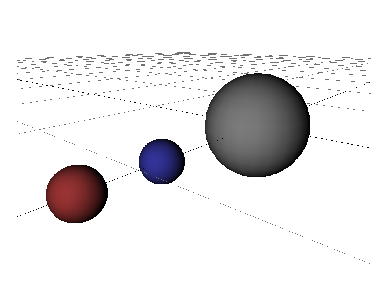
\epsfig{file=graphics/el_pr_de_white_small.eps}
	\caption{Elementarteilchen}
	\label{fig:Elementarteilchen}
\end{figure}

\subsection{Homogene Felder}

Um dem Aufrag gerecht zu werden und eine "`Computersimulation geladerner Teilchen in elektrischen und magnetischen Feldern"' zu erhalten, befinden sich nat�rlich auch homogene Felder im Reportua dieses Programms. Alle zu finden unter \textsl{Hinzuf�gen $->$ Homogene Felder}. Hier stehen dem Benutzer drei Feldarten zur Auswahl: Das elektrische Feld, das magnetische Feld und das Gravitationsfeld. Aufgrund ihrer homogenen Eigenschaft k�nnen diese �berall im Raum versetzt werden, ohne das es irgendeinen Einfluss auf das Geschehen nimmt. Wesentlich ist nur der Feldvektor, der mithilfe der \textsl{Channelbox} eingeblendet werden kann. Dieser l�sst sich wahlweise ebenfalls mit der \textsl{Channelbox} oder mit dem \textsl{Verschiebewerkzeug} zurecht drehen.
Auch das Drehen und Sklalieren des Wirkungsvektors eines Gravitationfeldes ist m�glich. Mit ihm lassen sich z.B. Perabelbahnen des freien Falls sehr sch�n darstellen. Zusammenfassend sind die homogenen Felder einfache Elemente, die ein relativ komplexeres System von z.B. Kondensatorplatten oder Helmholzspulenpaare stellvertretend ersetzen.

\begin{figure}[h]
	\centering
		\epsfig{file=graphics/Felder_white_small.eps}
	\caption{Homogene Felder}
	\label{fig:Homogene Felder}
\end{figure}


\subsection{Kondensatorplatte}

Da homogene Felder f�r manche Versuche nicht ausreichen k�nnten, weil sie z.B. einen unbegrenzten Wirkungsereich besitzen, kann das elektrische Feld auch durch zwei Kondensatorplatten ersetzt werden, welche ein inhomogenes Feld erzeugen. Das Verwenden von Kondensatorplatten ist allerdings ungleich komplizierter: Hier muss zun�chst die Anzahl der Aufteilungen bestimmt werden. Dies ist wichtig, damit das Programm wei�, mit wie vielen "`Ladungseinheiten"' es rechnen soll. Da ein Simulation von Milliarden positiver bzw. negativer Ladungen ein Ding der Unm�glichkeit w�r, beschrenkt sich dieses Programm auf eine geringere Anzahl, die der Benutzer selber angeben sollte. Die als Standartwert angegebenen zwei Aufteilungen eignen sich nicht besonders gut um das elektrische Feld eines Kondensators realistisch zu simulieren. Der Wert der hier zu w�hlen ist h�ngt von der Anzahl der Elementarteilchen ab, die sich in der Szene befinden und von der CPU-Leistung des Rechners, da dies bei Werten im dreistelligen Bereich sehr rechenaufw�ndig ist. Je h�her der gew�hlte Wert, desto genauer das inhomogene Feld und desto h�her s�mit der Realit�tgrad. Sobald eine neue Anzahl in der \textsl{Channelbox} eingegeben wurde, beginnt das Programm ein naturgem��e Verteilung der Elementarladungen. Dieser Vorgang kann dann durchaus 15 Minuten dauern und sollte nach dem endg�ltigen Skalieren der Platte manuell wiederholt werden.

\begin{figure}[h]
	\centering
		\epsfig{file=graphics/ladungsverteilung_white_small.eps}
	\caption{Kondensatorplatte}
	\label{fig:Kondensatorplatte}
\end{figure}


\subsection{"`Emitter"'}

Der Emitter (lat. emittere = aussenden; aussto�en) stellt eine flexible Elektronenkanone der Szene dar, welche dazu verwendet werden kann, andauernd Elektronen auszusenden. Der Vorteil dieses Instruments gegen�ber seines realen Gegenst�cks liegt in der Vielzahl der Einstellungsm�glichkeiten. Hier lassen sich neben der Position des Ger�ts auch Richtung und Betrag der auszusto�enden Teilchen angeben, und um wieviel von diesem Wert abgewichen werden darf. Da eine Elektronenkanone, bei der jedes Elektron genau den selben Geschwindigkeitsvektor bek�me, recht ausdrucksschwach w�re, weicht hier jedes Teilchen in der Startgeschwindigkeit um einen pseudozuf�lligen Vektor ab, der in der \textsl{Channelbox} unter den Feldern \textsl{Zufall X, Zufall Y und Zufall Z} indivieduell skaliert werden kann. Soll in einer Richtung keine Abweichung stattfinden ist hier der Wert Null einzugeben. Auch der zeitliche Abstand mit der die Ladungstr�ger das Ger�t verlassen l�sst sich manuell vorherbestimmen. Die Einheit des Abstand ist allerdings "`Frames\footnote{Bilder die am PC dargestellt werden}"' und nicht Sekunden oder sonst eine feste Zeiteinheit.

\begin{figure}[h]
	\centering
		\epsfig{file=graphics/Emitter_mit_Elektronenspur_white.eps}
	\caption{Emitter}
	\label{fig:Emitter_mit_Elektronenspur}
\end{figure}


\section{Halbschrittverfahren}

\subsection{Verfahren von Heun}

Ende des 19. Jahrhunderts besch�ftigte sich der Mathematiker und Philosoph Karl Heun mit der Berechung "`lnearer Differnzialgleichungen zweiter Ordnung, deren L�sungen durch den Kettenbruchalgortihmus verkn�pft sind"'\footnote{Quelle : http://www-history.mcs.st-andrews.ac.uk/Biographies/Heun.html}. Unter anderm beschrieb er dort auch einen Therm der es erm�glicht, eine relativ gute Ann�herung der Stammfunktion zu erhalten, wenn der Funktionstherm nur durch einzelne Werte beschrieben werden kann. Daher eignet er sich zum Beispiel gut bei der Berechnung von Planetenbahnen oder aber auch zur Berechnung Elementarteilchen in verschiedenen Feldern. Hier ist prinzipiell nur die Kraftwirkung gegeben, aus der dann �ber den Weg der Geschwindigkeit die Position des Teilchens bestimmt werden muss. Nach dem Hauptsatz der Integralrechnung ist also die Geschwindigkeit das Integral der Beschleunigung und die Position das Integral der Geschwindigkeit. Da die Beschleunigung jedoch nicht kontinuierlich berechnet wird, sondern nur alle X Millisekunden, l�uft man leicht Gefahr, dass die daraus berechneten Integrale stark von der Wirklichkeit abweichen. Diese Gefahr l�sst sich mit dem Verfahren von Heun zwar nicht vollst�ndig ausl�schen, aber dennoch stark minimieren.


\begin{center}
\begin{tabular}{|lcrcl|}

 	\hline &&&& \\
	Es sei gegeben die Funktion  & : & $ f(x) $ & $ = $ & $ m \cdot x + t$ \\ &&&& \\
	
	Auf Grund der Linearit�t & : &  $ f(x_{1} + \Delta x) $ & $ = $ & $ f(x_{1}) + f'(x_{1}) \cdot \Delta x $  \\ &&&& \\

	Daraus folgt nach Heun & : & 	$ f(x_{1} + \Delta x) $ & $ = $ & $ f(x_{1}) + \frac{f'(x_{1}) + f'(x_{1} + \Delta x) }{2} \cdot \Delta x $ \\ &&&& \\
	\hline
	 
\end{tabular}
\end{center}

Was f�r die lineare Funktion exakt gilt, wendet Heun als N�herung auch bei nicht linearen Funktionen an. Dieses Verfahren hat sich in der Praxis sehr bew�hrt und findet daher h�ufig bei Simulationen Anwendung, die keinen vollst�ndigen Funktionstherm besitzen \footnote{Quelle ( von 29.12.2007): http://www.acdca.ac.at/material/kl8/numerik.pdf}. \\
%\begin{figure}[h]
%	\centering
%		\epsfig{file=graphics/halbschrittverfahren.eps}
%	\caption{Halbschrittverfahren}
%	\label{fig:halbschrittverfahren}
%\end{figure}
\textbf{Am Rande bemerkt:} Carl Runge und Martin Wilhelm Kutta erweiterten das Verfahren von Heun, indem sie noch zus�tzlich in einem ganzen Schritt mehrere sogenannte "`St�tzpunkte"' verteilten und die Ableitungen an diesen dann zur Berechnung des Mittels einflie�en lie�en.

\begin{center}
\begin{tabular}{|ll|}

 	\hline & \\
	

	Heun& :	$ f(x_{1} + \Delta x) =  f(x_{1}) + \frac{f'(x_{1}) + f'(x_{1} + \Delta x) }{2} \cdot
		 \Delta x $ \\ & \\
		 
	Erweitert& :	$ f(x_{1} + \Delta x) = f(x_{1}) + \frac{f'(x_{1}) + 2 \cdot f'(x_{1} + \frac{1}{3} \cdot\Delta x)  + 2 \cdot f'(x_{1} + \frac{2}{3} \cdot\Delta x)+ f'(x_{1} + \Delta x) }{6} \cdot
		 \Delta x $ \\ & \\
		 
	Allgemein& :	$ f(x_{1} + \Delta x) = f(x_{1}) + \frac{f'(x_{1}) + 2 \cdot f'(x_{1} + \frac{1}{n} \cdot\Delta x)  + ... + 2 \cdot f'(x_{1} + \frac{n - 1}{n} \cdot\Delta x)+ f'(x_{1} + \Delta x) }{2 \cdot n} \cdot
		 \Delta x $ \\ & \\
	
	Kurz &:  $f(x_{1} + \Delta x) = f(x_{1}) + \frac{\Delta x}{2 \cdot n} \cdot ( \sum\limits^{n - 1}_{i = 0} f'(x_{1} + \frac{i}{n} \cdot\Delta x) + \sum\limits^{n}_{i = 1} f'(x_{1} + \frac{i}{n} \cdot\Delta x)) $ \\ & \\
         
		 
		 
	\hline
	 
\end{tabular}
\end{center}

%	Kurz : $$ f(x_{1} + \Delta x) = f(x_{1}) + \frac{1}{2 \cdot n} \cdot ( \sum^{n - 1}_{i = 0} f'(x_{1} + \frac{i}{n} \cdot\Delta x) + \sum^{n}_{i = 1} f'(x_{1} + \frac{i}{n} \cdot\Delta x)) \cdot \Delta x $$

\textbf{Bemerkung :} Die Zahl n ($ n \in \mathbbm{N} $) gibt die Anzahl der gesetzen St�tpunkte an.\\ \\


Da allerdings das Setzen von St�tzpunkten erneut eine Menge Rechenleistung des CPUs verbrauchen w�rde, wird dieses Verfahren in dieser Simulation nicht angewendet.

\subsection{Programiertechnische Anwendung}

Die Programiertechnische Anwendung gestaltet sich denkbar einfach: Man addiert zuerst die H�lfte der Ableitung multipliziert mit einer Konstante, berechnet dann die neuen Beschleunigungsvektoren und addiert zum Schluss den zweiten Teil der Ableitungen:


\tiny
\lstset{language=C++}
\lstinputlisting[breaklines=true, numbers=left, numberstyle=\tiny, firstline=601,  lastline=627 , frame=tlrb, caption={Quellcodeausschnitt aus einer bearbeitete Version von Physics.cpp, Zeile 601 - 627}]{Quellcode/bearbeitetePhysics.cpp}
\normalsize


\newpage

\section{Versuchsaufbauten}

\subsection{Wasserstoffatom}

Der einfachste Versuchsaufbau ist wohl ein Elektron, das um das 1000-fach schwerere Proton kreist. Nat�rlich ist dies nur eine primitive Vereinfachung des Wasserstoffatoms, welche alle bohrsche Quantenbedingungen und sonstige Atomvorstellung au�en vor l�sst. Zu sehen ist allerdings die Ellipsenbahn, auf der sich das Elekton bewegt:

\begin{figure}[h]
	\centering
	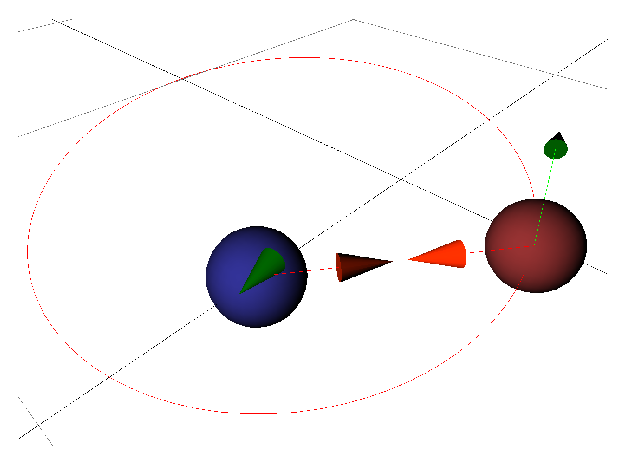
\epsfig{file=graphics/El_Pr_white.eps}
	\caption{Orbit-Versuch}
	\label{fig:Orbit-Versuch}
\end{figure}

Man beachte, dass jeweils die Impulse und die Kr�fte entgegengesetzt sind, und vom Betrag her gleich gro� sind.\\
(Dieser Versuch ist auf der CD unter dem Verzeichnis \textsl{Beispielszenen/H-Atom.sim} zu finden)

\subsection{Rutherford-Versuch}

Im Jahre 1911 beschoss Ernest Rutherford eine d�nne Goldfolie mit Alphateilchen. Aus diesen Ergebnissen begr�ndete er ein neues nach ihm benanntes Atommodell. Wenn man das Experiment genauer unter die Lupe nimmt, erkennt man, dass Rutherford positiv geladene Teilchen auf einen Atomkern schleuderte, welche von der \textsl{Coloumb-Kraft} abgelenkt wurden. Ersetzt man die Alphateilchen durch Elektronen und gibt dem Atomkern eine negative Ladung, l�sst sich auch die Rutherfordstreuung mit der Simulation zeigen.\\
(Zu finden auf der CD unter \textsl{Beispielszenen/RutherfordEx.sim})

\begin{figure}[h]
	\centering
		\epsfig{file=graphics/rutherfordEx_whiteEx.eps}
	\caption{Rutherfordstreuung}
	\label{fig:Rutherfordstreuung}
\end{figure}

\subsection{WIEN-Filter}

Ein ebenso interessanter Versuch ist der \textsl{Wien-Filter}. Dieses Ger�t wird in der experimentalen Physik dazu verwendet, Teilchen mit der falschen Geschwindigkeit aus einem Strahl heraus zu sieben. 

\begin{figure}[h]
	\centering
		\epsfig{file=graphics/wien_white.eps}
	\caption{WIEN-Filter}
	\label{fig:WIEN-Filter}
\end{figure}

Man beachte, dass die Bahn des Elektrons nicht exakt geradlinig ist, was daran liegt, dass die Anfangsgeschwindigkeit nicht 100-prozentig stimmt. Deshalb pendelt es immer zwischen der �bermacht der Lorenzkraft und der elektrischen Kraft.\\
(Zu finden auf der CD unter \textsl{Beispielszenen/wien-filter.sim})

\newpage

\section{Grenzen computergest�tzter Simulationen}

Doch leider wird man bei der Entwicklung computergest�tzter Simulationen immer wieder mit der Tatsache konfrontiert, wie schnell die begrenzte Rechenleistung eines Heim-PCs und die schwierige Beschreibung der Natur in manchen Teilbereichen jemanden an die Grenzen der physikalischen Simualtionstechnik treibt. Simulationen beispielsweise von Interferenzen an einem Doppelspalt w�rden bei einer �blich hohen Aufl�sung in Elementarwellen, die CPU-Leistung um ein Vielfaches �beranspruchen. Vor allem wenn es darum geht, ganze Volumina mit Werten zu f�llen, wie es z.B. bei dem Magnetfeld eines Helmholzspulenpaares der Fall w�re. Aus diesem und anderen Gr�nden wurde auf dieses Ger�t im Programm verzichtet. Allein das Ber�cksichtigen des Luftwiderstandes bei mechanischen Versuchen w�rde jede Computersimualtion den Gar ausmachen. Ebenfalls ist man nie davor gewappnet, irgendwelche Umwelteinfl�sse zu vergessen. Was die Frage der Verl�sslichkeit nicht zu gunsten der Simulationen beantwortet. Betrachtet man die hei�elbergsche Unsch�rferelation, dann w�ren die meisten Versuche mit Mirkoteilchen nicht mehr ganz so trivial zu beschreiben ,wie es der Computer mit seinen Schaltkreisen vermag.
Daher ist nicht jedes Gebiet der Physik gleich gut geeignet, es in ein PC-Programm zu verpacken.

%Hei�elbergsche Unsch�rferelation\\
%Sachen die mit einer Formel nicht greifbar sind
	
	%%
% Tabellen- und Abbildungsverzeichnis.
% Falls ben�tigt, einfach die %-Zeichen vor
% den Befehlen entfernen
%%
		%\listoftables
		\listoffigures
		\lstlistoflistings
		
		\vspace{1 cm}

\begin{Large}\textbf{Verwendete Quellen}\end{Large}

\begin{enumerate}
	\item  \hspace{0.5 cm}http://www.stmwfk.bayern.de/pressearchiv/meldung.asp?NewsID=649 \hfill 3
	\item  \hspace{0.5 cm}http://www.medien.ifi.lmu.de/fileadmin/mimuc/mll ws0506/Vortrag Kim.pdf \hfill 4
	\item  \hspace{0.5 cm}Physik, Leistugskurs 1. Semester, Seite 61  \hfill 8
	\item  \hspace{0.5 cm}Physik, Leistugskurs 1. Semester, Seite 110/111 \hfill 9
	\item  \hspace{0.5 cm}http://www-history.mcs.st-andrews.ac.uk/Biographies/Heun.html \hfill 14
	\item  \hspace{0.5 cm}http://www.acdca.ac.at/material/kl8/numerik.pdf \hfill 15
\end{enumerate}

	%%
	% Einbinden der Schlusserkl�rung
	
Ich erkl�re hiermit, dass ich die Facharbeit ohne fremde Hilfe angefertigt und nur die im Literaturverzeichnis angef�hrten Quellen und Hilfsmittel benutzt habe. \\ \vspace{2cm}

\begin{tabular}{p{5.5cm}p{3cm}lp{5cm}l}
\hrulefill , den		& \hrulefill 		&& \hrulefill\\
Ort 								& 	 Datum 			&& Unterschrift
\end{tabular}

\end{document}
